\documentclass[tikz,border=3pt]{standalone}
% common black-and-white style of the diagrams
\usepackage[T1]{fontenc}
\usepackage{mathptmx}
\usepackage{amsmath,amssymb,bm}
\usetikzlibrary{arrows.meta,positioning,fit,calc,backgrounds,shapes.geometric,shapes.misc,patterns}
\tikzset{
  every picture/.style={font=\small, line width=0.5pt},
  >={Latex[length=2.2mm,width=1.5mm]},
  blk/.style={draw, rectangle, fill=white, align=center, inner sep=3pt, minimum height=9mm},
  grp/.style={draw, rectangle, dashed, inner sep=4pt},
  arr/.style={->, line width=0.6pt},
  darr/.style={->, line width=0.6pt, dash pattern=on 3pt off 2pt},
  lbl/.style={font=\footnotesize, align=center},
  ttl/.style={font=\small\bfseries},
}

\AtBeginDocument{\hyphenpenalty=10000 \exhyphenpenalty=10000 \relax}

\begin{document}
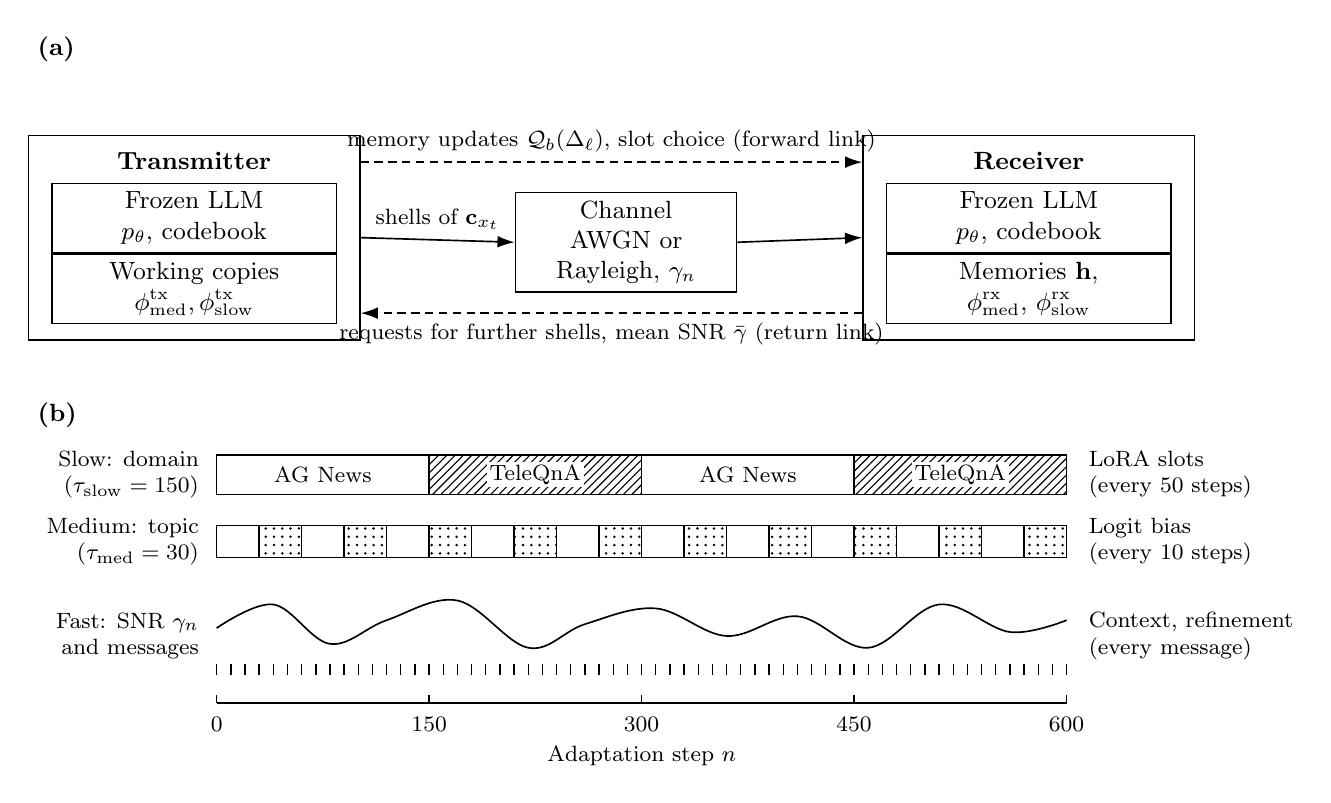
\begin{tikzpicture}
% ---------------- (a) link and information pattern
\node[ttl, anchor=west] at (0,4.3) {(a)};
\node[blk, text width=40mm, minimum height=26mm, anchor=south west] (txf) at (0,0.6) {};
\node[ttl, anchor=north] at ($(txf.north)+(0,-1mm)$) {Transmitter};
\node[blk, text width=34mm, minimum height=7mm] at ($(txf.center)+(0,0.25)$) {Frozen LLM $p_\theta$, codebook};
\node[blk, text width=34mm, minimum height=7mm] at ($(txf.center)+(0,-0.65)$) {Working copies $\phi^{\mathrm{tx}}_{\mathrm{med}},\phi^{\mathrm{tx}}_{\mathrm{slow}}$};
\node[blk, text width=40mm, minimum height=26mm, anchor=south west] (rxf) at (10.6,0.6) {};
\node[ttl, anchor=north] at ($(rxf.north)+(0,-1mm)$) {Receiver};
\node[blk, text width=34mm, minimum height=7mm] at ($(rxf.center)+(0,0.25)$) {Frozen LLM $p_\theta$, codebook};
\node[blk, text width=34mm, minimum height=7mm] at ($(rxf.center)+(0,-0.65)$) {Memories $\mathbf{h}$, $\phi^{\mathrm{rx}}_{\mathrm{med}}$, $\phi^{\mathrm{rx}}_{\mathrm{slow}}$};
\node[blk, text width=26mm, minimum height=11mm] (ch) at (7.6,1.85) {Channel\\ AWGN or Rayleigh, $\gamma_n$};
\draw[arr] ($(txf.east)+(0,0.0)$) -- node[lbl, above]{shells of $\mathbf{c}_{x_t}$} (ch.west);
\draw[arr] (ch.east) -- ($(rxf.west)+(0,0.0)$);
\draw[darr] ($(txf.north east)+(0,-0.35)$) -- node[lbl, above]{memory updates $\mathcal{Q}_b(\Delta_\ell)$, slot choice (forward link)} ($(rxf.north west)+(0,-0.35)$);
\draw[darr] ($(rxf.south west)+(0,0.35)$) -- node[lbl, below]{requests for further shells, mean SNR $\bar{\gamma}$ (return link)} ($(txf.south east)+(0,0.35)$);

% ---------------- (b) drift at three timescales
\node[ttl, anchor=west] at (0,-0.35) {(b)};
\def\x0{2.4}\def\L{10.8}
\pgfmathsetmacro{\u}{\L/600}
% slow band
\foreach \a/\b/\lab/\h in {0/150/AG News/0,150/300/TeleQnA/1,300/450/AG News/0,450/600/TeleQnA/1} {
  \ifnum\h=1
    \draw[pattern=north east lines] ({\x0+\u*\a},-1.35) rectangle ({\x0+\u*\b},-0.85);
    \node[fill=white, inner sep=1pt, font=\footnotesize] at ({\x0+\u*(\a+\b)/2},-1.1) {\lab};
  \else
    \draw ({\x0+\u*\a},-1.35) rectangle ({\x0+\u*\b},-0.85);
    \node[font=\footnotesize] at ({\x0+\u*(\a+\b)/2},-1.1) {\lab};
  \fi
}
% medium band: topic periods of 30 steps
\foreach \k in {0,...,19} {
  \pgfmathtruncatemacro{\odd}{mod(\k,2)}
  \ifnum\odd=1 \draw[pattern=dots] ({\x0+\u*30*\k},-2.15) rectangle ({\x0+\u*30*(\k+1)},-1.75);
  \else \draw ({\x0+\u*30*\k},-2.15) rectangle ({\x0+\u*30*(\k+1)},-1.75); \fi
}
% fast band: SNR trace and messages
\draw[line width=0.6pt] plot[smooth, tension=0.6] coordinates {
 ({\x0+\u*0},-3.05) ({\x0+\u*40},-2.75) ({\x0+\u*80},-3.25) ({\x0+\u*120},-2.95) ({\x0+\u*170},-2.7) ({\x0+\u*220},-3.3) ({\x0+\u*260},-3.0) ({\x0+\u*310},-2.8) ({\x0+\u*360},-3.15) ({\x0+\u*410},-2.9) ({\x0+\u*460},-3.3) ({\x0+\u*510},-2.75) ({\x0+\u*560},-3.1) ({\x0+\u*600},-2.95)};
\foreach \s in {0,10,...,600} { \draw ({\x0+\u*\s},-3.65) -- ++(0,0.15); }
% axis
\draw ({\x0},-4.0) -- ({\x0+\L},-4.0);
\foreach \s in {0,150,300,450,600} { \draw ({\x0+\u*\s},-4.0) -- ++(0,0.1); \node[font=\footnotesize, anchor=north] at ({\x0+\u*\s},-4.05) {\s}; }
\node[font=\footnotesize, anchor=north] at ({\x0+\L/2},-4.42) {Adaptation step $n$};
% left labels
\node[font=\footnotesize, anchor=east, align=right] at (\x0-0.1,-1.1) {Slow: domain\\ ($\tau_{\mathrm{slow}}=150$)};
\node[font=\footnotesize, anchor=east, align=right] at (\x0-0.1,-1.95) {Medium: topic\\ ($\tau_{\mathrm{med}}=30$)};
\node[font=\footnotesize, anchor=east, align=right] at (\x0-0.1,-3.15) {Fast: SNR $\gamma_n$\\ and messages};
% right labels: the memory that tracks each band
\node[font=\footnotesize, anchor=west, align=left] at (\x0+\L+0.15,-1.1) {LoRA slots\\ (every 50 steps)};
\node[font=\footnotesize, anchor=west, align=left] at (\x0+\L+0.15,-1.95) {Logit bias\\ (every 10 steps)};
\node[font=\footnotesize, anchor=west, align=left] at (\x0+\L+0.15,-3.15) {Context, refinement\\ (every message)};
\end{tikzpicture}
\end{document}
